\chapter{Tendencias y Estado del arte}

Antes de adentrarnos en el análisis del problema, debemos de tener en cuenta de que este problema es una temática en constante evolución, y por tanto, podemos encontrar diferentes conceptos y procedimientos seguidos en la literatura que pueden servirnos de inspiración para abordar el problema sin cometer los errores ya cometidos en el pasado, y ser capaces de encontrar un nuevo enfoque que nos ofrezca ventajas.\\

Generalmente, este problema ha sido abordado empleando hardware de computador de escritorio, por lo que la mayoría de modelos se centran en el aprovechamiento de los recursos hardware alojados en un servidor para realizar la clasificación y evaluación de las imágenes potencialmente cancerosas tomadas. Por tanto, nos adentraremos en sus conceptos, pero teniendo en cuenta que el proyecto propuesto hará uso de dispositivos móviles durante el tiempo de inferencia.

\section{Aprendizaje profundo en dispositivos móviles}

Con la creciente tendencia de la potencia de cálculo en los dispositivos actuales, prácticamente todos los aparatos electrónicos que nos rodean han crecido en cuanto a potencia y complejidad de cálculo. Los smartphones son precisamente uno de ellos, y nos acompañan cada día, por lo que es el dispositivo ideal para tareas de uso cotidiano y portabilidad.\\

Estos dispositivos, a diferencia de los computadores tradicionales, normalmente basado en la arquitectura x86 o AMD64, se basan en ARM, siguiendo como concepto de diseño ofrecer el máximo rendimiento posible dentro de unos consumos contenidos,mejorando el ahorro de energía y la pérdida de la misma mediante calor. El entrenamiento de modelos que encontramos habitualmente en la literatura, como ResNet, Inception o similares, es prácticamente inviable de forma nativa.\\

Sin embargo, en lo que respecta a la inferencia, éstos son capaces de ofrecer muy buenos resultados, gracias a la incorporación de hardware dedicado capaz de ofrecer estas características. Como prueba, podemos observar infinidad de aplicaciones que hace uso de ello, como Google Lens, que si bien se ayuda del uso de servidores de búsqueda especializados, es capaz de realizar procedimientos locales en los dispositivos de gama alta. \\

El objetivo del proyecto es aprovechar dicho vacío en la existencia de apliaciones de inferencia local para ofrecer una app que no necesite de conexión de red permanente para ofrecer resultados acerca de las manchas de piel identificadas.

\subsection{Arquitecturas neuronales de alta eficiencia}

Aprovechando el auge de los smartphones, grandes empresas, como Google y Meta, centran sus esfuerzos en la creación de arquitecturas basadas en redes convolucionales capaces en realizar detección de imágenes en tiempo real, para la clasificación de distintos objetos que podemos encontrar en nuestra vida cotidiana, y servir así como una herramienta de apoyo para diferentes necesidades. Sin embargo, esto es una tarea completa, ya que suelen carecer de complejas operaciones, o sacrificar en profundidad para lograr un rendimiento aceptable de unas decenas de milisegundos por inferencia.\\

A continuación, evaluaremos algunos de los modelos más conocidos y efectivos de propósito general, como SqueezeNet\cite{iandola2016squeezenet}, MobileNet \cite{howard2017mobilenets}\cite{sandler2019mobilenetv2}\cite{howard2019searching}, ShuffleNet \cite{zhang2017shufflenet} y  EfficientNet Lite \cite{tan2020efficientnet}\cite{eflite}.

\subsubsection{Squeeze-Net (2016)}

Squeeze-Net\cite{iandola2016squeezenet} se centra en la reducción de complejidad de la arquitectura, sin pérdida de capacidad predictiva y evitando aplicar técnicas de compresión y cuantización\cite{kuzmin2024fp8} de modelos. Se autodefine como ``una red al nivel de AlexNet\cite{NIPS2012_c399862d} pero con una quincuagésima parte de los parámetros'', haciendo alusión a disponer de una capacidad de cálculo similar a AlexNet, pero recortando en cuanto a número de parámetros necesarios.\\

Aunque el motivo de su creación no es de forma directa el uso de la arquitectura en dispositivos móviles, ha sido ampliamente utilizada en ellos al formar parte de la tendencia actual de reducción de coste computacional para reducir las necesidades de potencia de cálculo. De esta forma, se puede facilitar la implementación de redes convolucionales en sistemas empotrados con escasa capacidad de memoria y cómputo, haciendo uso de FPGAs \cite{fpga}.\\

Siguiendo este punto de vista, fue capaz de igualar e incluso superar levemente el rendimiento de AlexNet\cite{NIPS2012_c399862d}, empleando las siguientes técnicas:
\begin{itemize}
    \item Uso de módulos \textbf{Fire}. Se trata de un nuevo tipo de estructura convolucional modular que puede ser apilado en capas al estilo de los módulos Inception \cite{szegedy2014going} de Google. Consiste en una unidad modular ajustable en función de 3 parámetros: el número de convoluciones 1x1, y el número de filtros 1x1 y 3x3 de ``expasión'' a aplicar. El objetivo de añadir las convoluciones 1x1 es, por un lado, la reducción de dimensionalidad del volumen a convolucionar, y por otro lado, la simplificación en número de parámetros. En arquitecturas de gran profundidad, como VGGNet o ResNet, quedó demostrado que este tipo de convoluciones permitían llegar más allá sin perder información relevante para el aprendizaje. \ref{figsqueeze}
    \item Desplazamiento de los métodos de \textbf{reducción} de dimensionalidad hacia las capas más \textbf{profundas} de la arquitectura. En lugar de realizar pooling o aplicar stride a la hora de aplicar el filtro para reducir el volumen de salida en las primeras capas de la red, este tipo de transformaciones se reparten en capas más profundas para evitar que las capas cercanas al Head, de forma que se reduce la pérdida de características si retrasamos el subsampling del filtro.
    \item Eliminación de capas totalmente conectadas. Estas capas son, normalmente, las que mayor complejidad añaden al modelo por su gran cantidad de parámetros. Gracias al uso de Average Pooling en su última capa, podemos tener una red completamente independiente del tamaño de la entrada sin gran cantidad de parámetros ni necesidad de capas adicionales.
\end{itemize}

\begin{figure}[H]
	\label{figsqueeze}
	\centering
	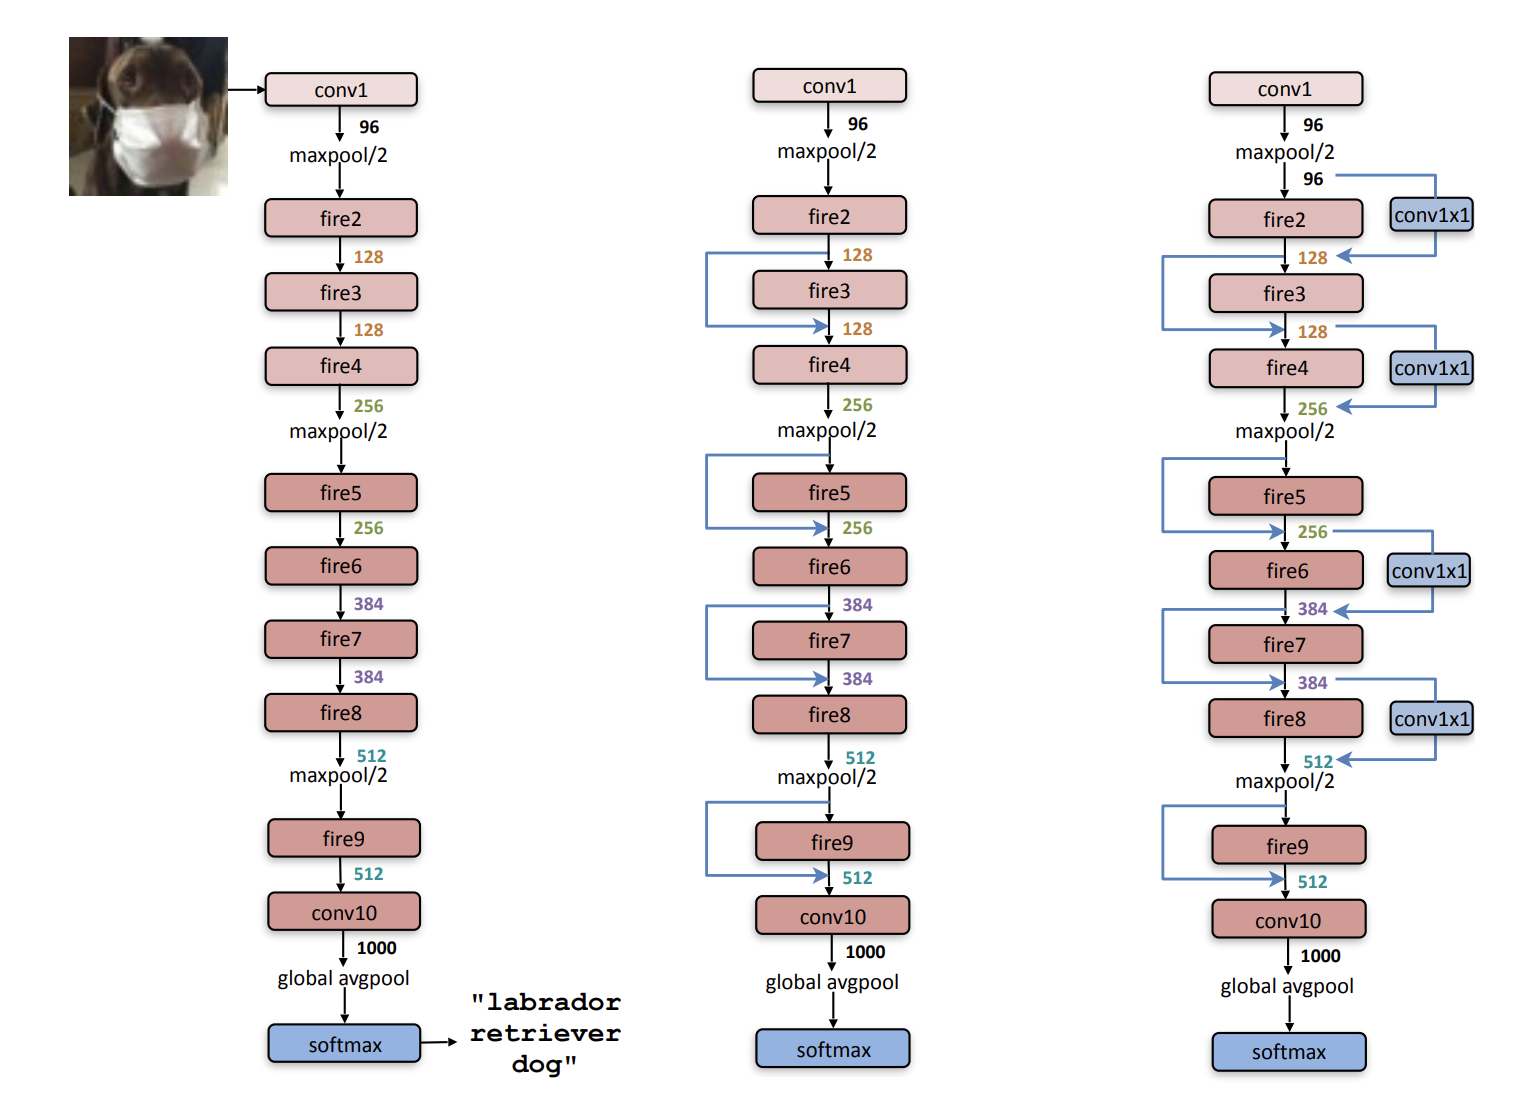
\includegraphics[scale = 0.2]{imagenes/squeezenet.png}
	\caption{Arquitectura de SqueezeNet}
\end{figure}


Esta red ha sido empleada en multitud de aplicaciones: detección de objetos en tiempo real, clasificación semántica, y modelos preliminares de conducción autónoma. Entre todas sus aplicaciones, podríamos destacar su utilización en imagen médica, concretamente MRI (Resonancias magnéticas). Ha permitido facilitar el diagnóstico de ciertas enfermedades y lesiones cerebrales en un espacio de memoria y recursos contenido.\\

Sin embargo, a pesar de las mejoras recibidas en sus versiones sucesivas, como los módulos Fire de doble nivel para reducir dimensionalidad, o la introducción de más reducciones mediante pooling, sacrifica resultados a nivel de accuracy respecto a la competencia, y no ha sido aplicada de forma firme y exitosa sobre imágenes de enfermedades cutáneas.



\subsection{MobileNet}

MobileNet es el fruto del proyecto de investigación de Google Research para la implementación de redes convolucionales en dispositivos móviles. El objetivo era encontrar un modelo eficiente que pueda ser incluso utilizado en tareas de segmentación en tiempo real, pero reduciendo el número de parámetros del red así como el número de operaciones de producto necesarias, para poder ejecutarlas de forma nativa en dispositivos móviles como smartphones y tablets.\\

Esta arquitectura consta de 3 versiones diferentes, siendo cada una más sofisticada que la anterior. Disponemos de MobileNet V1, MobileNet V2 y MobileNetV3.

\subsubsection{MobileNet V1 (2017)}

La versión original de la arquitectura convolucional MobileNet  \cite{howard2017mobilenets} fue publicada en 2017. En esta publicación, se busca reducir el número de operaciones realizadas para conseguir un menor impacto de las operaciones en punto flotante sobre el rendimiento.\\
El punto clave de esta arquitectura reside en las llamadas "pointwise convolutions", haciendo uso del concepto de separabilidad, ampliamente estudiado desde el año 2012 por la literatura.

Las nuevas convoluciones descomponibles se pueden separar en dos pasos bien delimitados: la convolución en profundidad y la convolución puntual.

\begin{itemize}
    \item Las convoluciones en profundidad realizan el producto del filtro con el volumen de entrada capa a capa. Es decir, no se tiene en cuenta la dimensionalidad total de la imagen, sino que se realiza por cada nivel de profundidad el mismo producto. Esto reduce considerablemente el número de parámetros, ya que la dimensionalidad del problema es mucho menor.
    \item La segunda fase es la convolución puntual, cuyo objetivo no es más que acumular el producto de todas las capas calculadas independientemente mediante una simple combinación lineal, la cual es de coste computacional muy bajo.
    
    $$G_{k,l,m} =  \sum_{i,j}^{} K^{i,j,m} * F_{k+i-1,l+j-1,m}$$
\end{itemize}

Este producto es calculable eficientemente por las técnica de álgebra lineal GEMM, que permite aplicar propiedades de la suma y la multiplicación para el producto matricial de forma eficiente mediante Tensor cores.\\

En resumen, gracias a la separabilidad convolucional, se adquieren varias ventajas:
\begin{itemize}
    \item El número de productos se reduce considerablemente. Como se puede verificar en \cite{howard2017mobilenets} se traduce en una reducción de entre 8 y 9 veces el número de operaciones con respecto a las arquitectura tradicional de convolución
    \item Se reduce el espacio necesario en memoria.
    \item Se puede aprovechar el hardware específico.
    \item No se pierde precisión de cálculo gracias a que la separabilidad de convoluciones no afecta al resultado.
\end{itemize}

\begin{figure}[H]
	\label{depthwise}
	\centering
	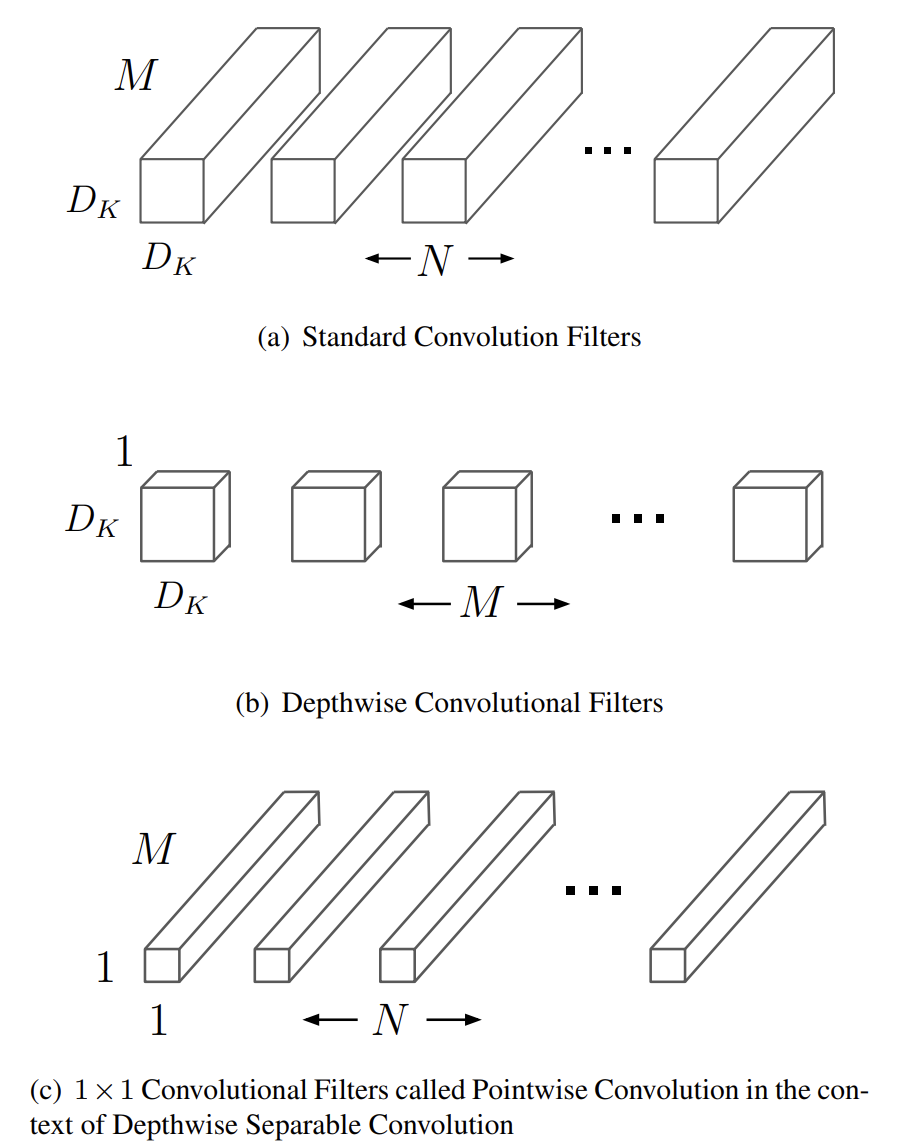
\includegraphics[scale = 0.225]{imagenes/depthwise.png}
	\caption{Producto depthwise}
\end{figure}

Adicionalmente, también incorporaron dos hiperparámetros: $\alpha$ y $\rho$. Estos parámetros controlan la anchura y la resolución de entrada, respectivamente.\\
El hiperparámetro $\alpha$ hace referencia a la anchura de cada capa convolucional que compone la red, adquiriendo un valor de 1 cuando la arquitectura no se ve reducida, y gradualmente podrá ser reducida en el intervalo (0,1]. Así se conseguirán modelos más simples en anchura para dispositivos con menores recursos.\\

En cuanto a $\rho$, este se encuentra implícito en la resolución de la imagen de entrada. Por defecto, la red acepta imágenes de hasta 224x224, pero en función de dicho valor $\rho$, podremos reducir su resolución también dentro del intervalo (0,1].\\

Ambos parámetros sacrificarán bondad y ajuste en los resultados a favor de una mayor eficiencia.

\subsubsection{MobileNet V2 (2018)}

Dos años más tarde de la publicación de MobileNets, da a luz su versión V2  \cite{sandler2019mobilenetv2}. Esta conserva los hiperparámetros  de la versión anterior, así como el producto punto a punto. Sin embargo, añade tres nuevas características, algunas de ellas no triviales y que requieren experimentación:
\begin{itemize}
    \item Se introduce el concepto de ``residuo invertido''. Ésta mejora reside en la utilización de los bloques residuales, propuesto por la arquitectura de ResNet. Su objetivo es evitar la degradación del gradiente, y que se frene el aprendizaje en modelos de gran profundidad. Normalmente, estas conexiones se realizan entre capas de gran profundidad, siendo las capas intermedias bloques estrechos. Sin embargo, en MobileNet V2, se propone la composición inversa, de forma que sean los bloques intermedios entre los residuales aquellos que poseen una mayor anchura, y así reducir el número de parámetros sin perder expresividad en el modelo \cite{invertedresidualsv2}.
    \begin{figure}[H]
    	\label{invert}
    	\centering
    	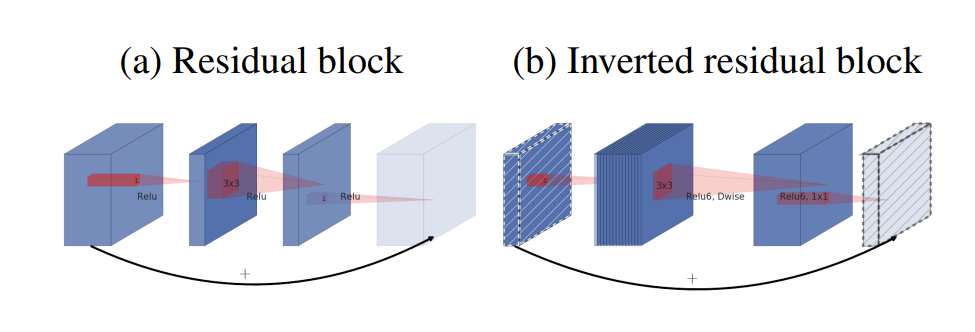
\includegraphics[scale = 0.3]{imagenes/invertedres.png}
    	\caption{Bloque residual invertido}
    \end{figure}
    
     \item En las capas donde el volumen de entrada es estrecho, al hacer uso de bloques residuales invertidos, la eliminación de la no linealidad aportada por ReLu favorece a la conservación de características y permite obtener mejores resultados de accuracy en tareas generales como clasificación en imagenet. Esto se debe a que al realizar los saltos entre bloques ``estrechos'' perdemos rendimiento de la red, y simplemente con eliminar la última transformación no lineal del bloque, contrarrestamos este problema.
    \item ReLu6. Se mantiene una versión modificada de la original función de activación. En lugar de utilizar la tradicional función ReLu entre 0 y 1, se extiende este intervalo hasta 6, permitiendo mantener la precisión en caso de utilizar coma fija, ya que se aseguran 3 dígitos de parte entera, y el resto queda destinado a la mantisa, que se almacena de forma precisa.
\end{itemize}

    \begin{figure}[H]
	\label{mv2}
	\centering
	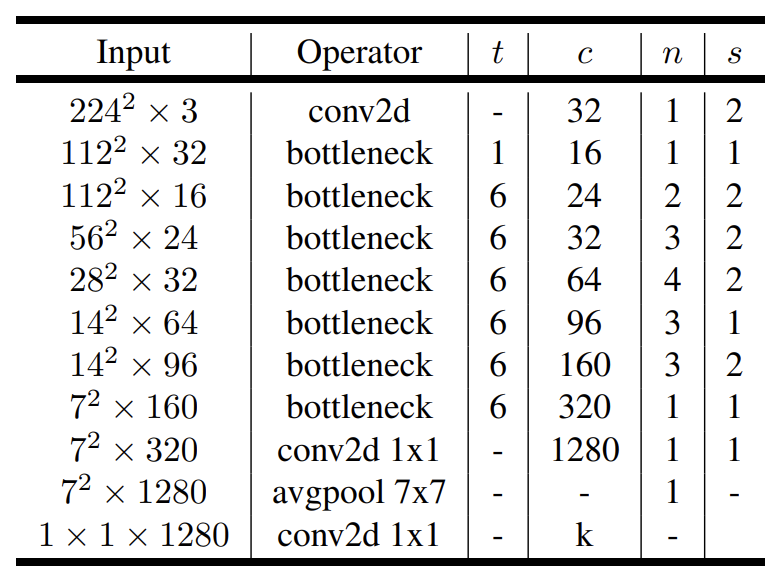
\includegraphics[scale = 0.25]{imagenes/mobilenetv2.png}
	\caption{Arquitectura de MobileNetV2}
\end{figure}

\subsubsection{MobileNet V3 (2019)}

En su tercera versión\cite{howard2019searching}, MobileNet incorpora métodos avanzados de diseños de redes basados en NetAdapt. Este algoritmo se basa en la transformación de modelos preentrenados para escritorio, y, en base a una serie de requisitos de potencia especificados, adapartar la arquitectura a una plataforma móvil perdiendo las mínimas capacidades posibles de la red original.  El modelo de partida empleado fue ajustado con precisión para mejorar latencias y uso de memoria, aplicando los siguientes conceptos:

\begin{itemize}
    \item Se añade la capa Squeeze-and-Excite, dentro de las conexiones residuales. Se trata de un mecanismo surgido en 2018 \cite{hu2019squeezeandexcitation}. Este estudio afirma que existen filtros de imagen con mayor importancia para el cómputo global que otros, como, por ejemplo, los bordes. Por tanto, les aporta un mayor ``peso'' durante el entrenamiento a dichos filtros haciendo uso de una serie de parámetros adicionales. Éstos añaden una carga computacional muy pequeña, por lo que se trata de una técnica eficaz. Para obtener los parámetros de relevancia, se dispone de dos módulos: squeeze, y excite. El módulo squeeze se encarga de representar cada filtro mediante un valor numérico, obtenido por average pooling de la imagen. Y por otro lado, el módulo excite se encarga de aprender los pesos que dar a cada uno de estos filtros o canales, haciendo uso de un MLP. El resultado final serán los pesos de cada canal en cuanto a su importancia, normalizados entre 0 y 1 por una función sigmoide.

    \item Se incluyeron nuevas capas al inicio y al final de la red de tipo residual invertidas.
\end{itemize}

    \begin{figure}[H]
	\label{mv2}
	\centering
	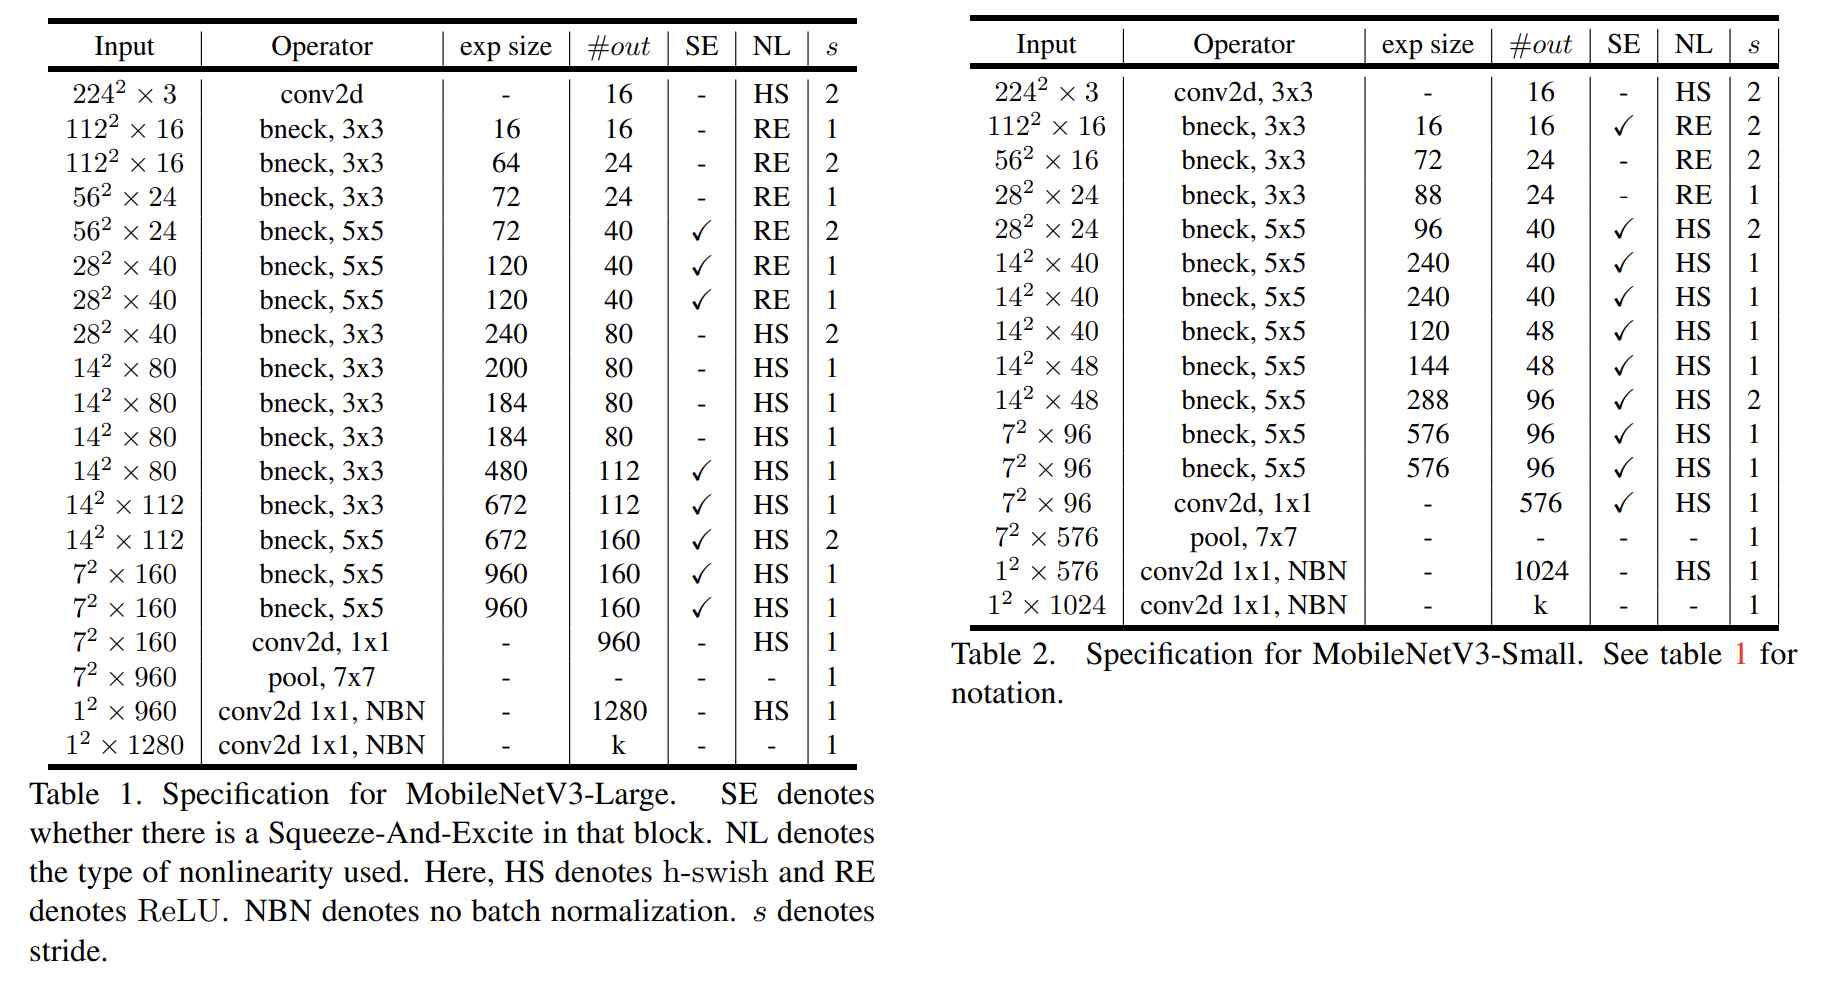
\includegraphics[scale = 0.85]{imagenes/mobilev3.png}
	\caption{Arquitectura de MobileNetV3}
\end{figure}

Debido a la gran complejidad adquirida por el modelo, los problemas de latencia y rendimiento en dispositivos de menor potencia, se opta por dividir la arquitectura en dos modelos parametrizables: MobileNet Small y Large. Mientras que la versión Large mejora los resultados de la versión 2 aumentando las prestaciones, el modelo Small otorga importancia sobre todo a la eficiencia y el uso de memoria, enfocado al hardware embebido o dispositivos de poca potencia.


\subsubsection{Aplicaciones en dermatología y cáncer de piel}

MobileNet, concretamente en su segunda versión, ha sido utilizado en la literatura para el diagnóstico de enfermedades de la piel. En \cite{Chaturvedi_2020}, es utilizado para realizar la clasificación de 7 enfermedades cutáneas extraídas del Humans against Machine, HAM10000 \cite{ham10000}, que podemos encontrar en ISIC archive \cite{isicarchive}, un repositorio web de acceso libre con enfermedades de la piel tanto beningnas como cancerosas. 

También se utilizó más recientemente para su implementación en dispositivos de IOT, \cite{mnetsqueeze}, donde se logra alcanzar el 99\% de accuracy en un pequeño conjunto extraido de ISIC, haciendo uso de la versión V3 junto a un algoritmo de Squeeze. Dicho algortimo se encarga de localizar la ubicación de los pelos y otros posibles artefactos para preprocesar la imagen y lograr una fotografía resultante libre de interferencias. 

Para ello, hace uso de un filtro black hat, que binariza la imagen y obtiene los píxeles objetivo de eliminar, que son sustituidos por los colores de los píxeles adyacentes, junto al uso del aumento de datos. Sin embargo, no queda especialmente claro la tasa de precisión del modelo para cada una de las enfermedades que se intentan diagnosticar.

\subsection{Shuffle Net}

Shuffle Net \cite{zhang2017shufflenet,shufflenetreview} surge con el objetivo ofrecer un modelo capaz de ofrecer un buen modelo con la mínima pérdida de rendimiento frente a modelos profundos. Es capaz de superar en resultados a la primera versión de MobileNet, logrando un error de aproximadamente tres puntos menos que MobileNet V1. Su mejor rendimiento se debe sobre todo al uso de Channel Shuffle para las convoluciones grupales, y creando una arquitectura basada en módulos shuffle.

La convolución en grupo mediante mezcla de canales (Channel Shuffle) surge tras el estudio del funcionamiento de las convoluciones grupales en 	AlexNet\cite{NIPS2012_c399862d} y ResNext. En ambos modelos, se uitilizan convoluciones grupales, donde cada canal de salida sólo se relaciona con los canales de entrada del que proviene. Esto podría debilitar la relación entre cada canal, y debilitar los resultados; para evitarlo, y no poner en riesgo el rendimiento con demasiadas convoluciones 1x1 para relacionarlos, se hace uso del mezclado de canales; es decir, es como si permitiésemos que cada grupo convolucional pudiera obtener información de otros grupos adyacentes, para así mejorar la relación entre ellos.

Para evitar un sistema complejo a la hora de representar dichas interconexiones, es como surge el channel shuffle \ref{shufflechannels}: se mezclan los canales de forma que los grupos ya no quedan aislados con sus respectivas entradas y salidas.

    \begin{figure}[H]
	\label{shufflechannels}
	\centering
	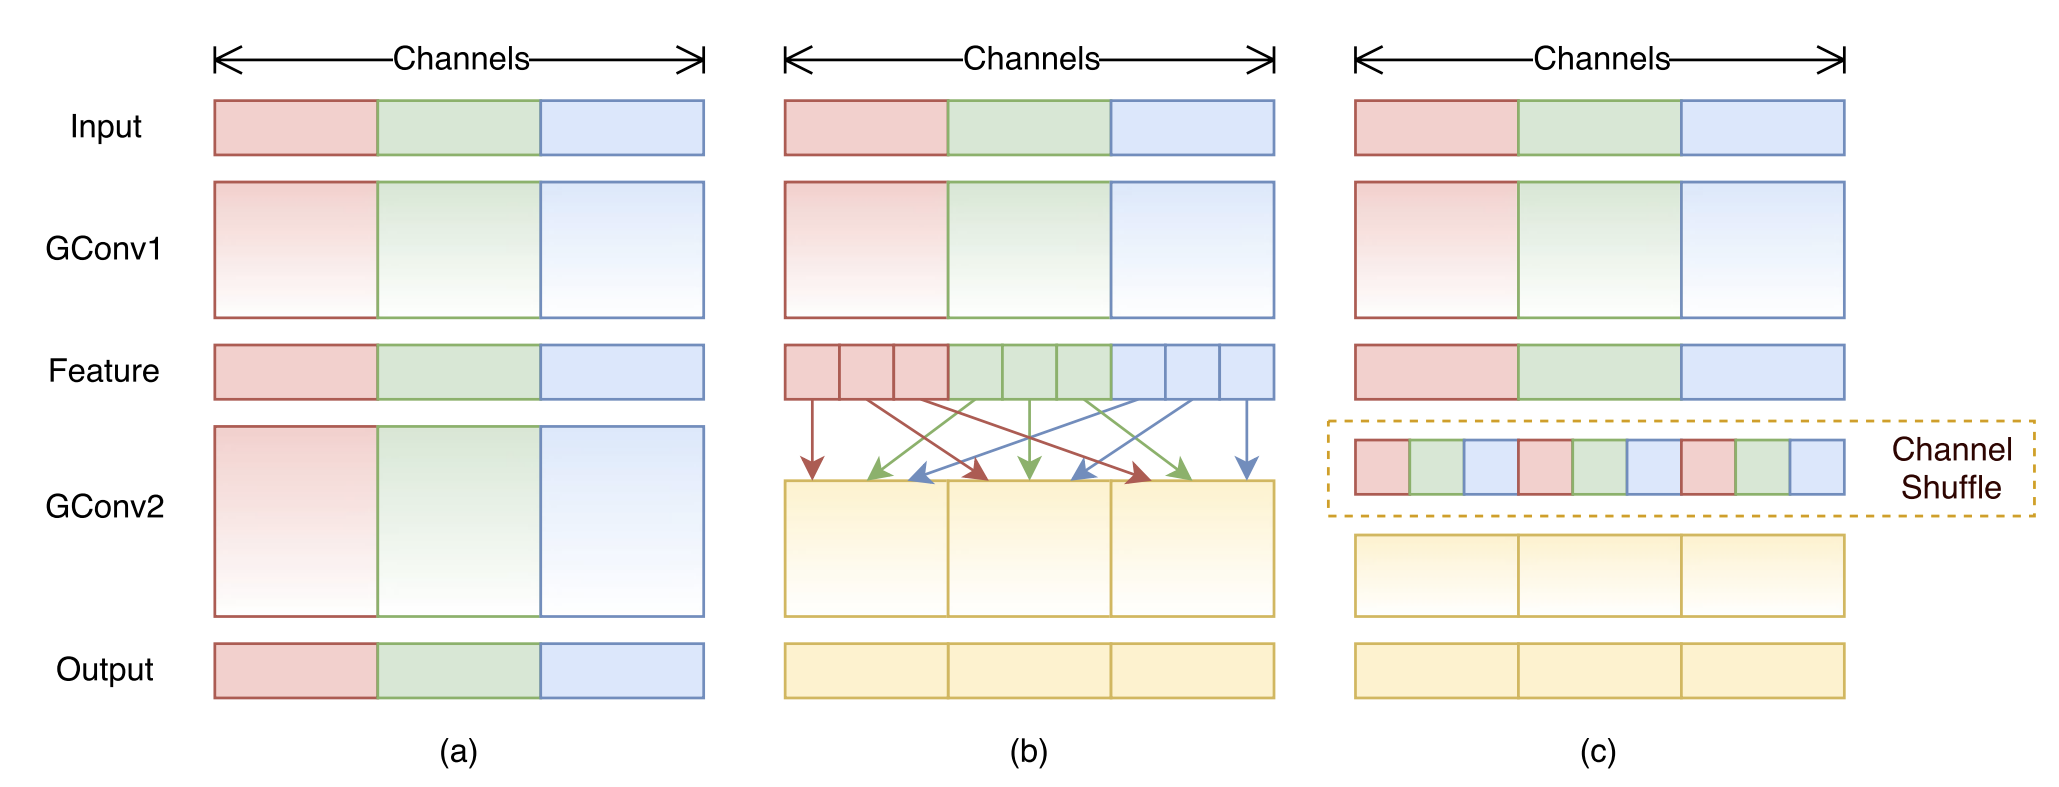
\includegraphics[scale = 0.2]{imagenes/shufflechannels.png}
	\caption{Channel Shuffle de ShuffleNet}
\end{figure}

Esta técnica se aplicará sobre la primera y última convolución 1x1 realizada sobre los bloques residuales de la red, que siguen una estructura parecida a la que adoptaría MobileNetV2 posteriormente. Mediante esta propuesta, podemos además aplicar una mayor capacidad de procesamiento en anchura añadiendo stride, y aplicando average pooling. El resultado, es conseguir modelos más anchos en procesamiento que no impacten negativamente en el rendimiento de los dispositivos con menor capacidad. En la figura \ref{label} , podemos apreciar la arquitectura de la red, cuyos filtros pueden ser escalados mediante el parámetro s, aunque teniendo en cuenta una penalización en la complejidad, equivalente a $s^2$ sobre Shuffle Net base, equivalente a $s=1$

\begin{figure}[H]
		\label{arquitecturashuffle}
		\centering
		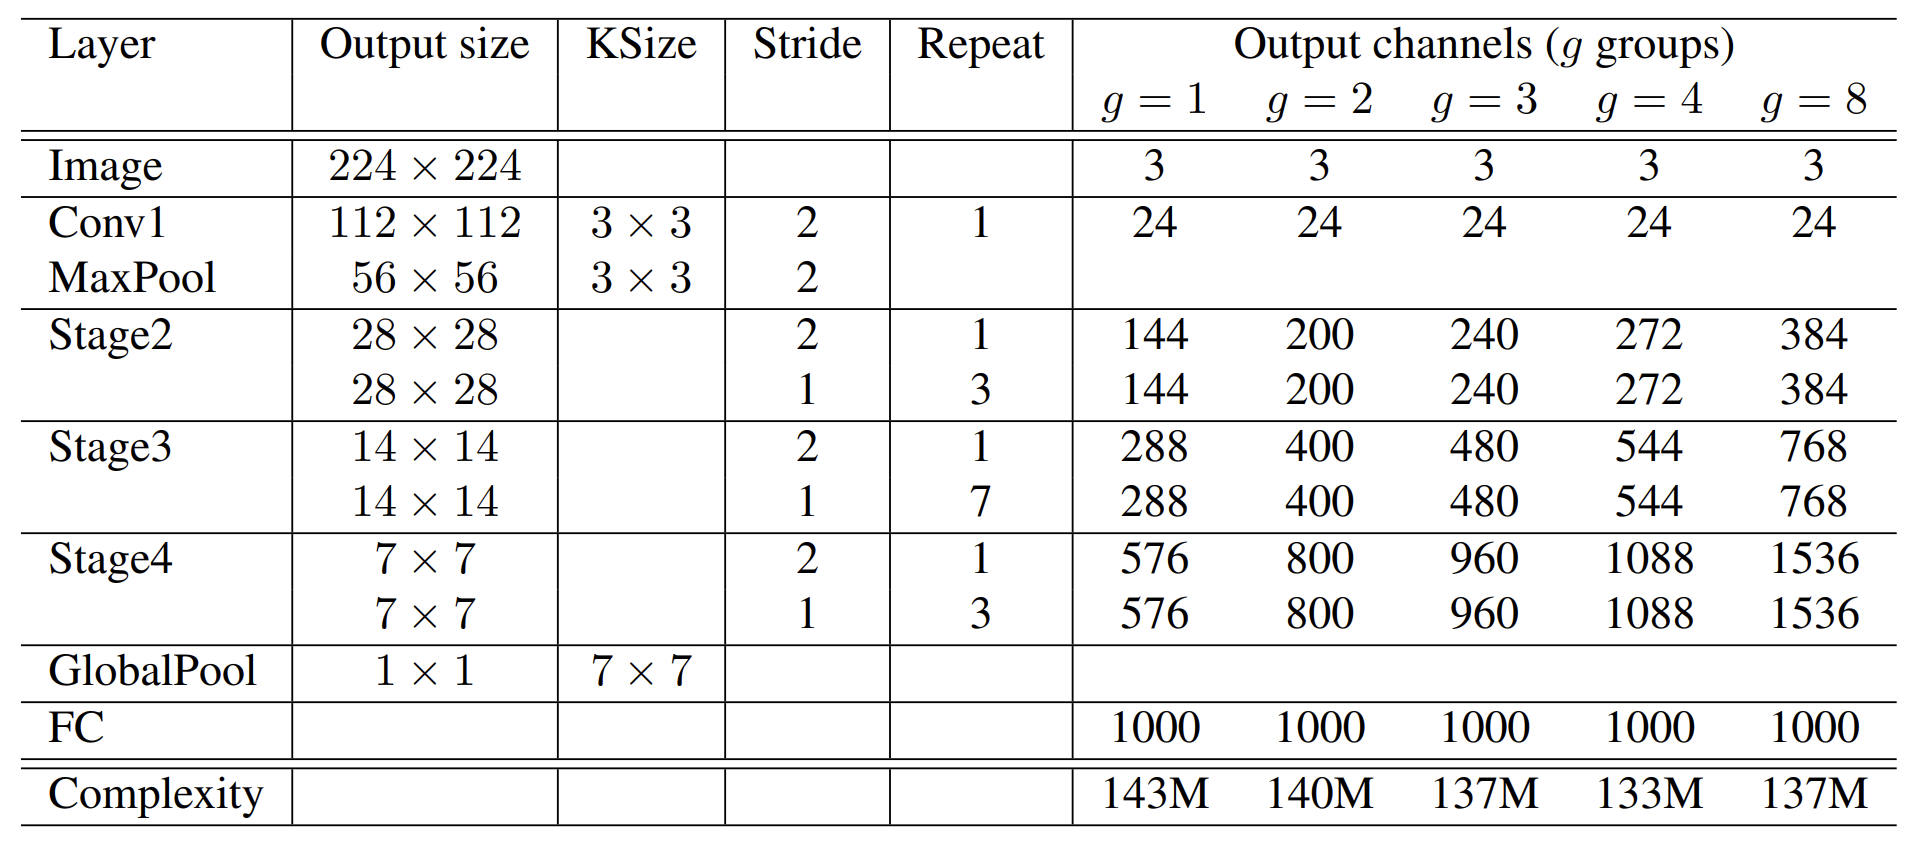
\includegraphics[scale = 0.2]{imagenes/arquitecturashuffle.png}
		\caption{Arquitectura de ShuffleNet}
	\end{figure}

Sus aplicaciones han sido variadas, pero en lo que respecta a la detección de lesiones cutáneas, la cercana salida de MobileNet V2 y su mejor rendimiento provocó que ShuffleNet quedase relegada a un segundo plano, y no fuese muy utilizada para este fin. Podemos encontrar algunos trabajos \cite{shuffleapp} donde podemos observar una comparativa de este modelo frente a la completitud de los modelos del estado del arte de 2022, y podemos confirmar que  MobileNetV2 es capaz de superar su rendimiento en la mayoría de pruebas, siendo estas comparaciones en cuanto a tiempo de entrenamiento, precisión, accuracy y tamaño del conjunto de entrenamiento. Sólo consigue superar a MobileNetV2 en tiempo de entrenamiento, donde es aproximadamente 900 más rápida, pero ofrece peores resultados en promedio.

\subsection{EfficientNet lite}

EfficientNet \cite{Chaturvedi_2020} es un conjunto de arquitecturas de redes creadas por el departamento de investigación de Google con el fin de conseguir una familia de modelos variada que fuese capaz de adaptarse fácilmente mediante parámetros a diferentes conjuntos de imágenes, y a requisitos de hardware más o menos limitados. 

Parte de que una red convolucional sigue el siguiente esquema:
$$\mathcal{N}=\odot_{i=1...s} F_i^{L_i}(X_{(H_i, W_i,L_i)})$$


Donde se denota que la capa $F_i$ es repetida $L_i$ veces la etapa i de la red, y la dimensionalidad de la capa queda representada con ${( W_i,L_i)}$.  Fijando $F_i$, efficient net intenta dar versatilidad a sus modelos variando las dimensiones restantes, Li, Ci, Hi, Wi mediante el uso de 3 constantes de escalabilidad:

\begin{itemize}
	 \item  Profundidad, Depth (d):  Aumentar la profundidad es la tendencia habitual presente en las redes convolucionales. Pero llegar a un equilibrio es crítico, ya que aumentar demasiado la profundidad sin modificar otros parámetros puede ocasionar pérdidades rendimiento por el desvanecimiento del gradiente  a menor profundidad. 
	\item Anchura, Width (w): Aumentar la anchura suele ser beneficioso para modelos de pocos recursos donde el aumento de profundidad supone un gran aumento de la carga computacional. Permite conseguir mayor cantidad de características de grado fino, pero si la red es demasiado poco profunda, el modelo careceré de características de alto grado que permitan aprender patrones generales.
	\item Resolución, (r): al emplear tamaños de entrada mayores, damos opciones a obtener una mayor cantidad de características de grado fino, pero un exceso de resolución puede provocar grandes tiempos de ejecución y puede ser contraproducente, al reducirse la ganancia con tamaños demasiados grandes.
\end{itemize}

\begin{figure}[H]
	\label{arquitecturashuffle}
	\centering
	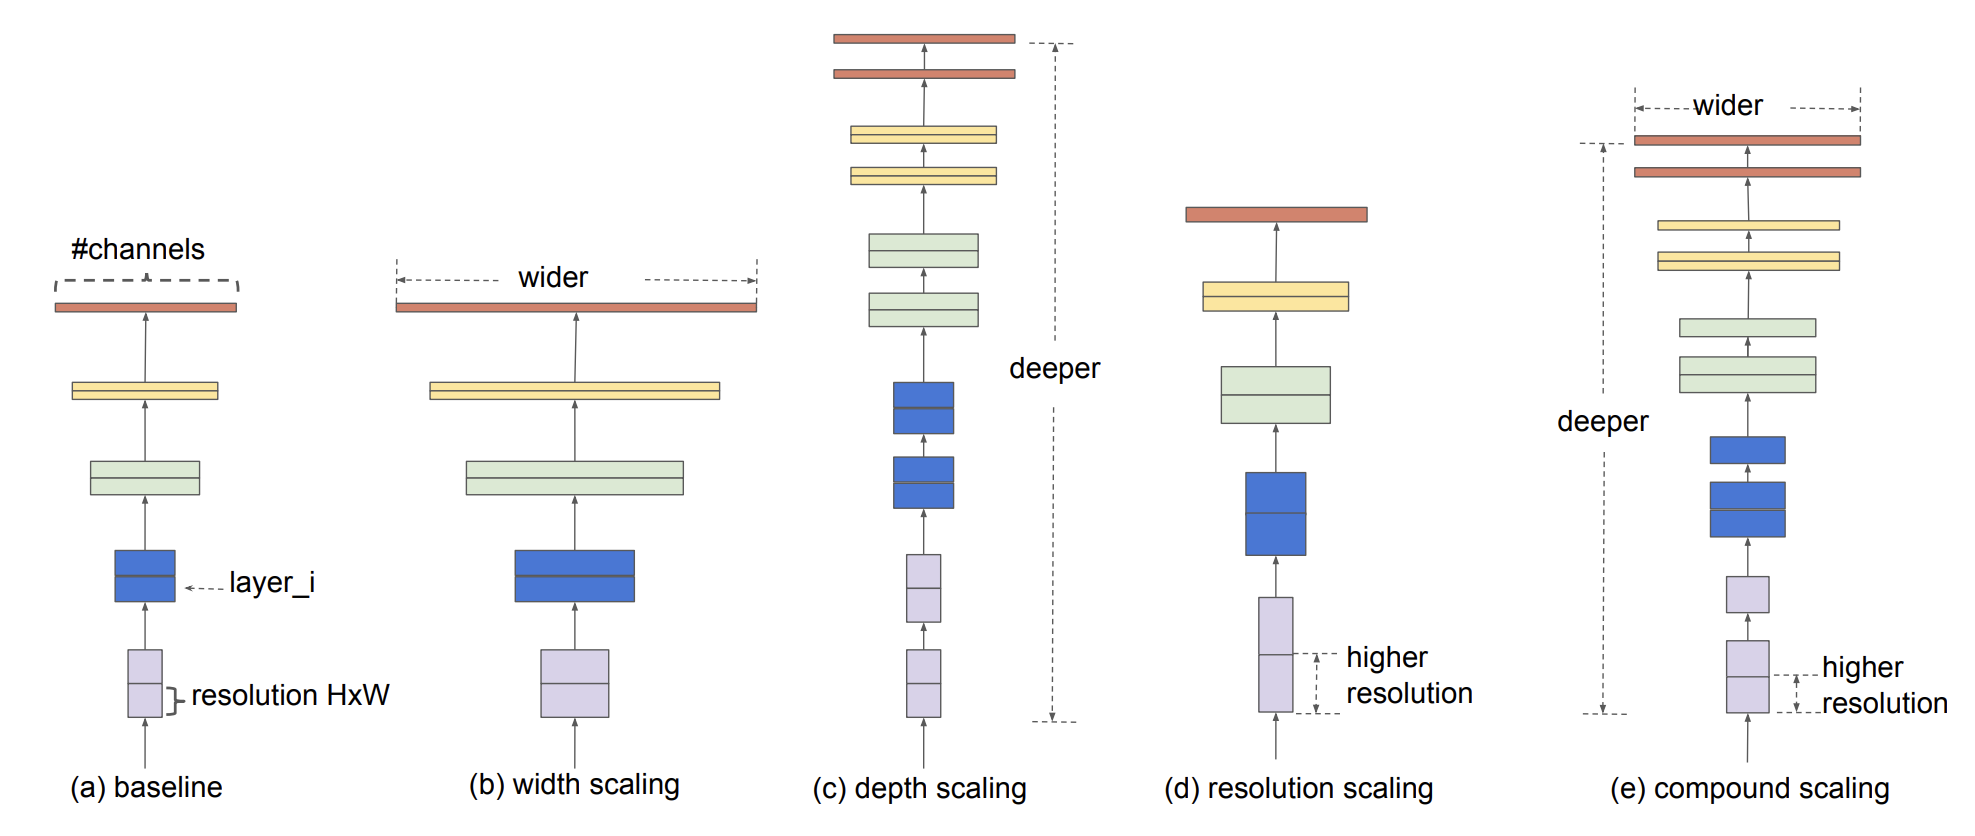
\includegraphics[scale = 0.2]{imagenes/efnet_scale.png}
	\caption{Parámetros de EfficientNet}
\end{figure}


Experimentalmente, estos parámetros pueden ser ajustados, y dan lugar a una serie de modelos distinto: los conocidos EfficientNetB0 - B7, denotando el valor numérico la profundidad y complejidad del modelo, siendo esta mayor a mayor valor del índice.	 Cada una de ellas fue ajustada utilizando como requisito la potencia medida en TFLOPS para su ejecución, y puede ser posteriormente ajustada con el resto de parámetros libres no fijados a las características del conjunto de entrada.\\


\subsubsection{Aplicaciones en dermatología y cáncer de piel}

En el problema que nos concierne, esta arquitectura ha conseguido grandes resultados en el dataset del ISIC abierto al público como competición en la plataforma Kaggle, habiendo sido utilizado como parte de un ensemble de modelos, o bien como modelo único entrenado en el top 3 de ganadores de la competición. En el caso de la segunda mejor solución clasificada \cite{2ndISIC}, se menciona la utilización de EfficientNet-B6, con tamaño de entrada de 512x512, y un tamaño de batch de 64, obteniendo 0.9485 de accuracy como resultado final a la hora de emplear los datasets ISIC 2019 y 2020\\ En la primera solución, es usada en conjunto a Resnet50, y una red especializada en los metadatos de la imagen, y todos los modelos juntos someten su resultado a votación \cite{1stISIC}.

Ambos resultados han sido evaluados con computadores de alta gama, haciendo uso de múltiples tarjetas gráficas para el entreanmiento y la inferencia. Este proceso es demasiado pesado para un dispositivo móvil, por lo que de cara a este trabajo, se buscarán alternativas capaces de ahorrar en espacio y potencia como concepto de cuantización.

 \subsection{Cuantización de modelos}


\section{Recursos gráficos disponibles}

La obtención de datos es un proceso fundamental en la resolución de problemas de Machine Learning. Este tipo de problemas requieren un gran número de imágenes que aporten variedad, y permitan construir un modelo general que se capaz de adaptarse a cambios de iluminación, diferentes puntos de vista y composiciones.

Es clave, por tanto, disponer de diferentes tipos de lesiones, tanto benignas como malignas, así como diferentes tonos de piel. La inexistencia de un tipo de piel en el conjunto de entrenamiento, o la inexistencia de un tipo de lesión podrían provocar resultados sesgados indeseados durante la predicción de la imagen tomada.

Podemos encontrar en la red varios datasets de acceso público que permiten su utilización de forma abierta con fines académicos. Dada a la gran cantidad de publicaciones disponibles, resulta complejo averiguar si los datos a los cuales hace referencia se encuentran disponibles públicamente, si son de acceso restringido, o bien, ya no se encuentran disponibles debido a cambios en su política o la falta de mantenimiento.

Debido a que el estudio de la evolución y el diagnóstico del cáncer de piel de forma temprana es un tema en auge, existen gran cantidad de publicaciones especializadas únicamente en el análisis de los conjuntos de datos públicamente accesibles, como es el caso de la lista propuesta por M. Goyal et Al. [16], o el reciente estudio realizado por Sana Nazari y Rafael García (2023)[30].
Basados en su modelo de estudio y las referencias recomendadas por sus artículos, se ha elaborado el siguiente plan de búsqueda para saber qué tipo de datos utilizar y cuáles descartar:

\begin{figure}[H]
	\centering
	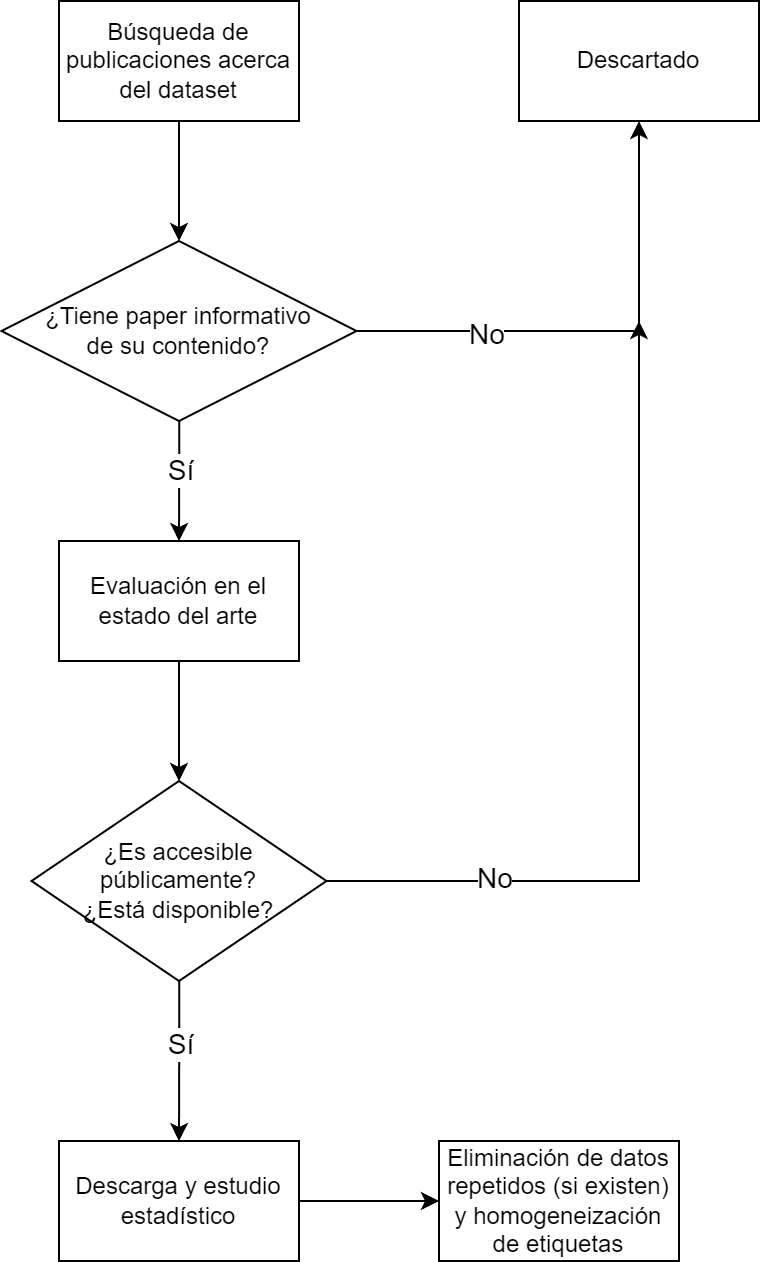
\includegraphics[scale=0.75]{imagenes/DiagramaBusqueda.png}
	\caption{Proceso de búsqueda seguido}
\end{figure}

Siguiendo dicho procedimiento, se han encontrado 6 datasets diferentes, cuyo origen son instituciones públicas que han cedido datos con fines académicos y de investigación.\\

Un factor determinante para la elección de estos conjuntos es la diversidad. Es indispensable, para este proyecto, encontrar datos lo suficientemente variados como para distinguir lesiones cancerígenas y no cancerígenas, y disponer de diferentes tonos de piel para entrenar. Aunque los tonos de piel más oscuras sufren lesiones de tipo cancerígeno en menor proporción gracias a su protección natural, también pueden sufrir este tipo de patologías, y es clave ser capaces de detectarlas en cualquier posible paciente.

\subsubsection{ISIC Data}
El repositorio ISIC (International Skin Imaging Collaboration [1]), contiene imágenes demoscópicas de lesiones principalmente cancerosas.  Existe una gran cantidad de publicaciones acerca de este conjunto de datos, debido a su utilización anual durante los años 2016-2020 para la realización de un reto virtual de Machine Learning descrito en [1]. El objetivo, consiste en identificar los melanomas frente a lesiones no cancerosas (ISIC Challenge-2020[2]) o bien, identificar diferentes subtipos de lesiones cancerosas frente a lesiones benignas (ISIC Challenge 2019, [3]). \\

En el estado del arte, destacan las soluciones que hacen uso de métodos de DeepLearning, como el planteado por Ian Pan [4], finalista de la competición para el año 2020. El ganador de la competición del año 2020, cuyo análisis podemos encontrar en [5], realiza por su parte un enfoque híbrido entre el uso de DeepLearning para la clasificación de los datos de tipo imagen, y clasificación mediante Machine Learning para los metadatos, y así obtener un resultado más preciso. \\

Debido a que cada uno de estos subconjuntos de datos anuales podían ser pequeños, normalmente se recurría a la reutilización de los conjuntos anteriores para enriquecer el conjunto de entrenamiento.  Este método es bastante recomendable, ya que, a mayor conjunto de entrenamiento, más cercanos se encontrarán los parámetros de interés del problema general a solucionar. Sin embargo, hay que realizar dicha fusión con especial cuidado, ya que existen volúmenes de datos considerables que se repitieron en las competiciones de cada año para aumentar el tamaño del dataset, y si se realizase una simple concatenación de los datos, estaríamos desperdiciando esfuerzo computacional en clasificar imágenes redundantes (comportamiento para nada deseable al trabajar sobre entornos móviles de menor potencia.).\\

Un análisis extenso de los datos asociados a cada Challenge podemos encontrarlo en [6]. En él, se recogen otros modelos del estado del arte utilizables para este fin, así como una forma de tratar los datos duplicados. Los datos pueden ser separados en los siguientes subconjuntos:

\begin{table}[H]
	\centering
	\begin{tabular}{|l|l|l|l|l|}
		\hline
		\textbf{Challenge Dataset Year} & \textbf{Train} & \textbf{Test} & \textbf{Total} & \textbf{Tipo de problema } \\ \hline
		ISIC 2016 & 900 & 379 & 1279 & Clas. binaria  \\ \hline
		ISIC 2017 & 2000 & 600 & 2600 & Clas. Multiclase  \\ \hline
		ISIC 2018 & 10015 & 1512 & 11527 & Clas. Multiclase  \\ \hline
		ISIC 2019 & 25331 & 8238 & 33569 & Clas. Multiclase  \\ \hline
		ISIC 2020 & 33126 & 10982 & 44108 & Clas. Binaria  \\ \hline
	\end{tabular}
\end{table}

\begin{itemize}
	
	\item ISIC 2016 [7]:  Es el dataset de menor tamaño de todos los propuestos. Hace distinción únicamente de los casos malignos y benignos. Contiene imágenes dermoscópicas anotadas con información acerca de la localización de la mancha, y la edad del paciente. Contiene información adicional para la segmentación de la mancha pigmentada de interés (máscaras).
	\item ISIC 2017 [8] Es un conjunto de mayor tamaño al anterior, y hace alusión a 4 clases diferentes: melanomas, nevus, y seborrheic keratosis. Contiene también información acerca de la edad del paciente, y otros metadatos de interés. La escasa cantidad de datos provoca que normalmente en la literatura este dataset se utilice también como clasificación binaria entre nevus y keratosis, u otros enfoques similares. 
	\item ISIC 2018 [9]. Este dataset contiene un número de imágenes considerables, siendo un total de 10015 imágenes para entrenamiento, y 1512 para test. En este caso, se realiza subclasificación de tipos, a través de las clases melanocytic nevus, basal cell carcinoma, actinic keratosis, benign keratosis, dermatofibroma y lesiones vasculares. Es de especial interés destacar que este dataset proviene, a su vez, de HAM10000 (Human against machine, [11] )  y MSK Dataset [12]. El challenge original comprendía, de nuevo, la clasificación de los diferentes tipos realizando previamente una discriminación de la mancha en cuestión mediante segmentación. Existen gran cantidad de publicaciones que tratan este conjunto de datos, como [13], donde se emplea este dataset para demostrar mejores resultados al emplear transformaciones polares de la imagen y aumentar la invarianza.
	
	\item ISIC 2019 [2].  Se trata del mayor conjunto de datos para clasificación multiclase propuesto por ISIC [1]. Se trata del mismo dataset que el año 2018 [9], con la adición de BCN\_20000 Dataset [14], cuyos datos provienen del Hospital Clínic de Barcelona [14]. Las clases a clasificar se amplían hasta 9, encontrando subtipos de melanomas en el conjunto.
	\item ISIC 2020 [3]. El último dataset propuesto públicamente, contiene únicamente datos binarios acordes a melanomas y no malignos. 
\end{itemize}

Todos estos datos pueden ser acoplados entre sí para dar un dataset global de ISIC [6], donde obtendríamos las siguientes clases: 


\begin{table}[H]
	\centering
	\begin{tabular}{|c|c|c|c|c|}
		\hline
		\textbf{Clase} & \textbf{2017} & \textbf{2018} & \textbf{2019} & \textbf{2020} \\ \hline
		\textbf{Melanoma} & 374 & 1113 & 4522 & 584 \\ \hline
		\textbf{Atypical melanocytic proliferation} & - & - & - & 1 \\ \hline
		\textbf{Cafe-au-lait macule} & - & - & - & 1 \\ \hline
		\textbf{Lentigo NOS} & - & - & - & 44 \\ \hline
		\textbf{Lichenoid keratosis} & - & - & - & 37 \\ \hline
		\textbf{Nevus} & - & - & - & 5193 \\ \hline
		\textbf{Seborrheic keratosis} & 254 & - & - & 135 \\ \hline
		\textbf{Solar lentigo} & - & - & - & 7 \\ \hline
		\textbf{Melanocytic nevus} & - & 6705 & 12.875 & - \\ \hline
		\textbf{Basal cell carcinoma} & - & 514 & 3323 & - \\ \hline
		\textbf{Actinic keratosis} & - & 327 & 867 & - \\ \hline
		\textbf{Benign keratosis} & - & 1099 & 2624 & - \\ \hline
		\textbf{Dermatofibroma} & - & 115 & 239 & - \\ \hline
		\textbf{Vascular lesion} & - & 142 & 253 & - \\ \hline
		\textbf{Squamous cell carcinoma} & - & - & 628 & - \\ \hline
		\textbf{Other / Unknown} & 1372 & - & - & 27.124 \\ \hline
		\textbf{Total} & 2000 & 10.015 & 25.331 & 33.126 \\ \hline
	\end{tabular}
\end{table}

Sin embargo, sería necesario tener en cuenta la eliminación de imágenes repetidas, debido a que durante cada edición de ISIC, un número considerable de imágenes han sido incluidos en varios años. Este procedimiento engloba:

\begin{enumerate}
	
	
	\item Eliminar las imágenes idénticas por hash. Todas las imágenes de ISIC están numeradas de forma única para facilitar la identificación de cada una de ellas. Si unimos todos los datatesets, y tomamos las repeticiones, podemos remover:
	
	\begin{table}[H]
		\centering
		\begin{tabular}{|c|c|c|c|c|c|}
			\hline
			\textbf{} & \textbf{2016} & \textbf{2017} & \textbf{2018} & \textbf{2019} & \textbf{2020} \\ \hline
			\textbf{Train} & 291 & 1283 & 0 & 0 & 0 \\ \hline
			\textbf{Test} & 95 & 594 & 0 & 0 & 0 \\ \hline
		\end{tabular}
		\caption{Número de imágenes duplicadas recogidas por [6]}
	\end{table}
	
	
	\item 	Eliminación del ISIC 2018. Como éste se encuentra contenido en la composición para el año 2019, puede prescindirse totalmente de él a favor de la versión de 2019.
	\item 	Eliminación de imágenes “downsampled” del conjunto. En los años 2019 y 2020, se añadieron imágenes de challenges anteriores con una reducción en resolución. Para ahorar en espacio y tiempo de cómputo, pueden eliminarse las imágenes reducidas para quedarnos con una única copia de mayor calidad de la lesión, y luego realizarles manualmente un reescalado en caso de que sea necesario.
	
	Atendiendo de nuevo a los resultados propuestos por [6], obtenemos el siguiente conjunto: 
	
	\begin{table}[H]
		\centering
		\begin{tabular}{|c|c|c|c|}
			\hline
			\textbf{Year} & \textbf{Task No.} & \textbf{Images Removed} & \textbf{Images Remaining} \\ \hline
			\textbf{2016} & 3 & 826 & 74 \\ \hline
			\textbf{2017} & 3 & 801 & 1199 \\ \hline
			\textbf{2018} & 3 & 10,015 & 0 \\ \hline
			\textbf{2019} & 1 & 2235 & 23,096 \\ \hline
			\textbf{2020} & - & 433 & 32,693 \\ \hline
			\textbf{Total} & - & 14,310 & 57,0621 \\ \hline
		\end{tabular}
		\caption{Tabla de imágenes únicas extraída de [6]. En este caso, el autor descarta el uso del dataset de 2016 por su baja aportación}
	\end{table}
	
\end{enumerate}

Obtendríamos un total de 57000 imágenes, los cuales podrían clasificarse, con sus respectivas clases extraídas de los metadatos. Componen, en resumen, un conjunto de datos robusto que puede formar parte del dataset de entrenamiento de este trabajo.
\begin{figure}[H]
	\centering
	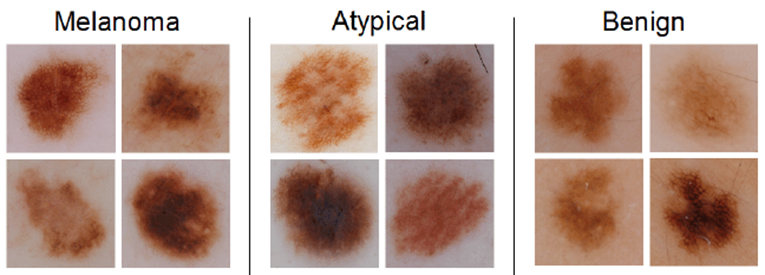
\includegraphics[scale = 0.5]{imagenes/Ejemplo2020.png}
	\caption{Ejemplo de imágenes de ISIC 2017 [23]}
	\label{fig:enter-label}
\end{figure}

\subsubsection{ASAN Dataset}

ASAN (Seung Seog Han 2018)[15][18][19] es un conjunto de datos de origen surcoreano compuesto por lesiones malignas y benignas de la piel. Nos permite obtener un mayor grado de variedad de las imágenes, ya que el repositorio ISIC se centra sobre todo en lesiones de piel de población europea. 

\begin{table}[H]
	\centering
	\begin{tabular}{|c|c|}
		\hline
		\textbf{Tipo de lesión} & \textbf{Número de ejemplares} \\ \hline
		{Actinic keratoses and intraepithelial carcinoma (AKIEC)} & 651 \\ \hline
		{Basal Cell Carcinoma (BCC)} & 1082 \\ \hline
		{Dermatofibroma (DF)} & 1247 \\ \hline
		{Hereditary angioedema (HAO)} & 2715 \\ \hline
		{Intraepithelial Carcinoma (IC)} & 918 \\ \hline
		{Lentigo (LEN)} & 1193 \\ \hline
		{Melanoma (ML)} & 599 \\ \hline
		{Nevus (NV)} & 2706 \\ \hline
		{Pyogenic Granuloma (PG)}  & 375 \\ \hline
		{Squamous Cell Carcinoma (SCC)} & 1231 \\ \hline
		{Seborrhoeic Keratosis (SK)}  & 1423 \\ \hline
		{Wart} & 2985 \\ \hline
		\textbf{Total} & \textbf{17125} \\ \hline
	\end{tabular}
	\caption{Distribución de clases de ASAN dataset}
\end{table}

Tal y como se describe en [17] (M Goyal 2019), este dataset tiene 12 tipos de enfermedades, sumando un total de 17125 imágenes clínicas. Estas imágenes están compuestas en su mayoría por imágenes en miniatura, pero existe un repositorio con imágenes de mayor tamaño, donde sería necesario realizar tareas de segmentación- Sin embargo, dichas imágenes son de acceso restringido, y se requieren permisos especiales del hospital para acceder a ellos. Por ese motivo, tendremos únicamente en cuenta loas 17125 miniaturas.

Adicionalmente, podemos encontrar también imágenes proporcionadas por Hallym, un dataset complementario de 125 imágenes pertenecientes a lesiones de tipo melanoma cancerosas.

Las clases más destacadas de este dataset en su conjunto son la presencia de lesiones benignas de la piel, detalle que no encontramos en ISIC, y que permiten así contrastar información de la piel con lesiones benignas con la piel cancerosa. Podemos encontrar 4 clases benignas: lentigos (manchas solares fruto del envejecimiento y la exposición prolongada al sol), nevus (lunares comunes), verrugas y granulomas benignos. 

\begin{figure}[H]
	\centering
	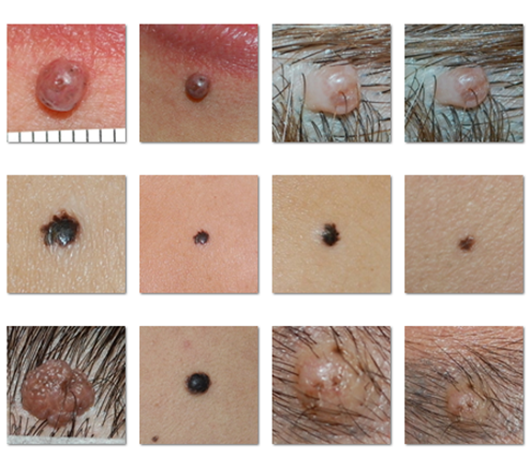
\includegraphics[scale = 0.6]{imagenes/ASAN.png}
	\caption{Ejemplo de lunares beningnos en ASAN (Nevus)}
\end{figure}

Los resultados han sido confirmados por expertos dermatólogos y los resultados verificados en su mayoría mediante biopsia, por lo que las etiquetas asociadas a cada lesión están completamente verificadas.\\

El formato de las imágenes es una disposición matricial de las miniaturas, donde cada fichero que contiene las subimágenes representa en su conjunto una clase. Por desgracia, no se aporta otro tipo de información adicional más allá de la etiqueta por motivos de privacidad.

\subsubsection{Dermnetz}

Podemos encontrar extraer este dataset de un atlas online de enfermedades cutáneas recogidas de pacientes alrededor de todo el mundo. Contiene tanto lesiones benignas como malignas, existiendo además manchas y lesiones vinculadas a enfermedades infecciosas y hongos. 

Existen gran cantidad de herramientas para realizar esta extracción de datos, como la que podemos encontrar en [21]. En total, se pueden obtener hasta 23000 imágenes, existiendo un total de 23 clases no balanceadas. Podemos encontrar lesiones de tipo alérgico, así como acné, dermatitis severa o celulitis.

Carece de metadatos asociados, ya que dicha información es de carácter reservado por su mantenedor.  El dataset no se encuentra listo para usar de forma inmediata, ya que desde 2019, las imágenes deben ser extraídas de la propia web, pues dispone un índice donde se pueden acceder a las enfermedades de interés. El fichero contenedor del dataset fue retirado en 2019 del libre acceso, junto a sus metadatos. Es necesario solicitar su acceso y aportar una cantidad económica.


\subsubsection{ PH2}
El conjunto de datos PH2 [22] es un conjunto de 200 imágenes obtenidas gracias al hospital Pedro Hispano de Portugal. Está compuesto por imágenes de alta resolución que contienen 3 posibles casos de lesiones:
\begin{itemize}
	\item Lunar común (Common Nevus), 80 ejemplares
	\item Lunar atípico (Atypical Nevus), 80 ejemplares
	\item Melanomas, 40 ejemplares.
\end{itemize}

Además de las 200 imágenes, podemos encontrar metadatos asociados a cada una de ellas, como el color, su extensión, textura, forma del borde, localización, entre otros.
Su acceso es libre para fines académicos desde su página oficial [22], que contiene las imágenes en formato jpg, y varios ficheros .csv con la información de la imagen y su clasificación.

\begin{figure}[H]
	\centering
	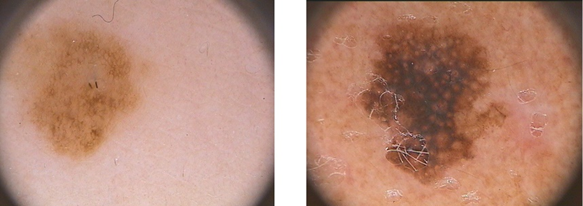
\includegraphics[scale = 0.6]{imagenes/PH2.png}
	\caption{Nevus maligno y benigno en PH2}
\end{figure}

\subsubsection{PAD-UFES 20}

PAD-UFES-20 [25] se trata de un conjunto de datos recopilado de diferentes poblaciones, que contiene diagnósticos para 1.641 lesiones cutáneas únicas recopiladas, comprendiendo un total de 2.298 imágenes.\\

Entre sus clases, podemos encontrar tres enfermedades y tres cánceres de piel.  Todos estos datos han sido recogidos y verificados mediante biopsia en un 100\% de los casos cancerosos, por lo que su diagnóstico está totalmente verificado.\\

Podemos encontrar, además del diagnóstico, metadatos acerca de:
\begin{itemize}
	\item ID de paciente
	\item ID de lesión, 
	\item ID de imagen
	\item Si la lesión benigna fue o no probada por biopsia.
	\item Información del paciente: fumador o no, localización de la lesión, edad, exposición a químicos, historial cancerígeno, etc.
\end{itemize}
Los datos han sido recogidos mediante teléfonos móviles en formato PNG, siendo las imágenes validadas por el Hospital Pathological Anatomy Unit of the University Hospital Cassiano Antȳnio Moraes (HUCAM) de la Federal University of Espírito Santo (Brasil). 
En su publicación original [25], podemos encontrar un resumen de su contenido de forma más específica:

\begin{table}[!ht]
	\centering
	\begin{tabular}{|c|c|c|}
		\hline
		\textbf{Diagnostico} & \textbf{Ejemplares} & \textbf{\% biopsied} \\ \hline
		Actinic Keratosis (ACK) & 730 & 24.4\% \\ \hline
		Basal Cell Carcinoma of skin (BCC) & 845 & 100\% \\ \hline
		Malignant Melanoma (MEL) & 52 & 100\% \\ \hline
		Melanocytic Nevus of Skin (NEV) & 244 & 24.6\% \\ \hline
		Squamous Cell Carcinoma (SCC) & 192 & 100\% \\ \hline
		\textbf{Total} & \textbf{2298} & \textbf{58.4\%} \\ \hline
	\end{tabular}
	\caption{Tabla de casos diagnosticados en PAD-UFES20}
\end{table}

Donde podemos apreciar que todos los casos de enfermedades cancerígenas han sido probados mediante biopsia, y el cáncer de célula basal se trata del tipo de enfermedad más frecuente.

\begin{figure}[H]
	\centering
	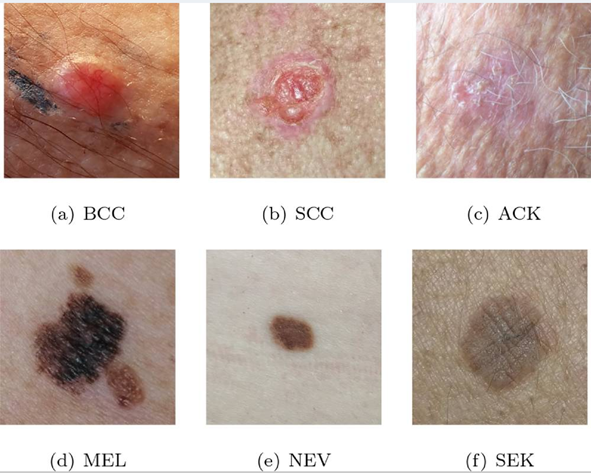
\includegraphics[scale = 0.45]{imagenes/PAD-UFES.png}
	\caption{Batch de ejemplo de PAD-UFES 20 [25]}
\end{figure}

\subsubsection{Severance}
Se trata de un conjunto de imágenes de lesiones cutáneas [24] recopiladas de pacientes de Corea del Sur. Recibe dicho nombre a que los datos recopilados cuentan con la colaboración del Hospital Severance, en el mismo país. \\

En su variante A, que es la única disponible públicamente, podemos encontrar el diagnóstico y otra información asociada sobre 10426 imágenes, cuya valoración se encuentra entre las 38 posibles clases que contiene este conjunto de datos. \\

Seleccionando las 6 clases más comunes contenidas en este dataset, encontraremos que comprenden aproximadamente el 75\% del conjunto. Está compuesto por actinickeratosis (22.5\%), angiofibromas (14.4\%), angiokeratomas(13.8\%), cáncer de tipo basal cell (8.1\%), Becker nevus (7.5\%), bluenevus (6.2\%), y la enfermedad de Bowen (carcinomas)(6.1\%).

El interés en este dataset se debe a que algunas de estas clases mayoritarias, como los nevus azules y de Becker, son condiciones benignas que suelen ser retirados únicamente con fines estéticos, permitiendo complementar con el resto de los diagnósticos negativos. Este tipo de lunares son los más complejos de diagnosticar, debido a sus colores similares a un melanoma, y suelen requerir una biopsia, por lo que su diagnóstico suele alargarse.

Las imágenes se encuentran en formato matriz, por lo que es necesario proceder a su separación previo a su utilización con fines de Deep Learning: 

\begin{figure}[H]
	\centering
	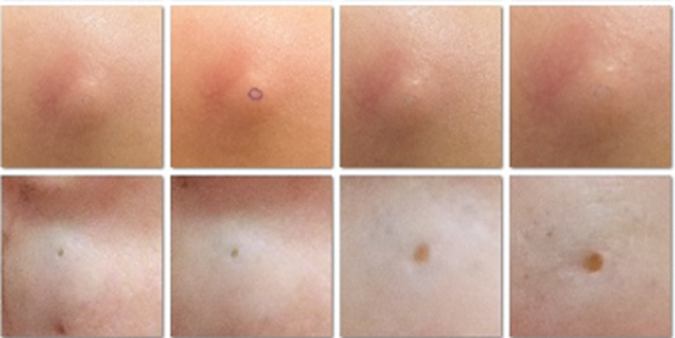
\includegraphics[scale = 0.5]{imagenes/Severance.png}
	\caption{Imágenes de ejemplo provenientes del dataset Severance   }
\end{figure}

\subsubsection{Otros datasets}
Existen otros datasets ampliamente referenciados que son de acceso público. Sin embargo, en los últimos años, éstos han sido retirados y han quedado inaccesibles. Es el caso de DermQuest, un atlas virtual que contenía lesiones cutáneas y otras patologías. Ese dataset fue contenido posteriormente por Derm101, pero ambas versiones fueron retiradas para su descarga. Alternativamente, podemos encontrar algunas de sus imágenes en los datasets SD-198 y SD-260 [26][29], pero únicamente permanece en activo el primero de ellos, bajo solicitud. En total, SD-198 contiene más de 6500 imágenes, mientras que SD-260 alcanzaba las 20000 imágenes.

En el estado del arte actual, podemos encontrar otros datasets ampliamente utilizados, como el caso de DermIS [27], un atlas online de patologías de la piel. También existen publicaciones reciente sobre nuevos conjuntos de datos utilizados de uso restringido, que permiten observar que la tendencia de investigación de este campo sigue en alza; es el caso del estudio propuesto por Papadakis et Al (2021) [28], que recoge datos sobre pacientes con melanoma de grado 3 para estudiar su evolución durante un período de 3 años, para estimar su crecimiento y potencial grosor del tumor.

Debido a las restricciones de acceso, ninguno de estos datasets será empleado como parte del entrenamiento del modelo diseñado para este estudio.

\subsubsection{Conjunto resultado}
Una vez examinados todos los conjuntos mencionados anteriormente, podemos llevar a cabo la unión de todos los datos en un único subconjunto. Esto nos permitirá conseguir un dataset completo y variado con diferentes tipos de piel y diferentes lesiones que nos permitirán identificar multitud de tipos de patologías, siendo posible ajustar el grado de granularidad en función de la agrupación o no de posibles subclases.

Inicialmente, el conjunto de datos construido contendrá todos los subtipos de lesiones cutáneas vistos, pero dispondrán de una segunda etiqueta que indicará si se trata de un caso canceroso o no, atendiendo a su subclase que lo etiqueta. Si agrupamos por lesiones benignas, cancerosas, y potencialmente cancerosas, obtenemos:


\begin{figure}[H]
	\centering
	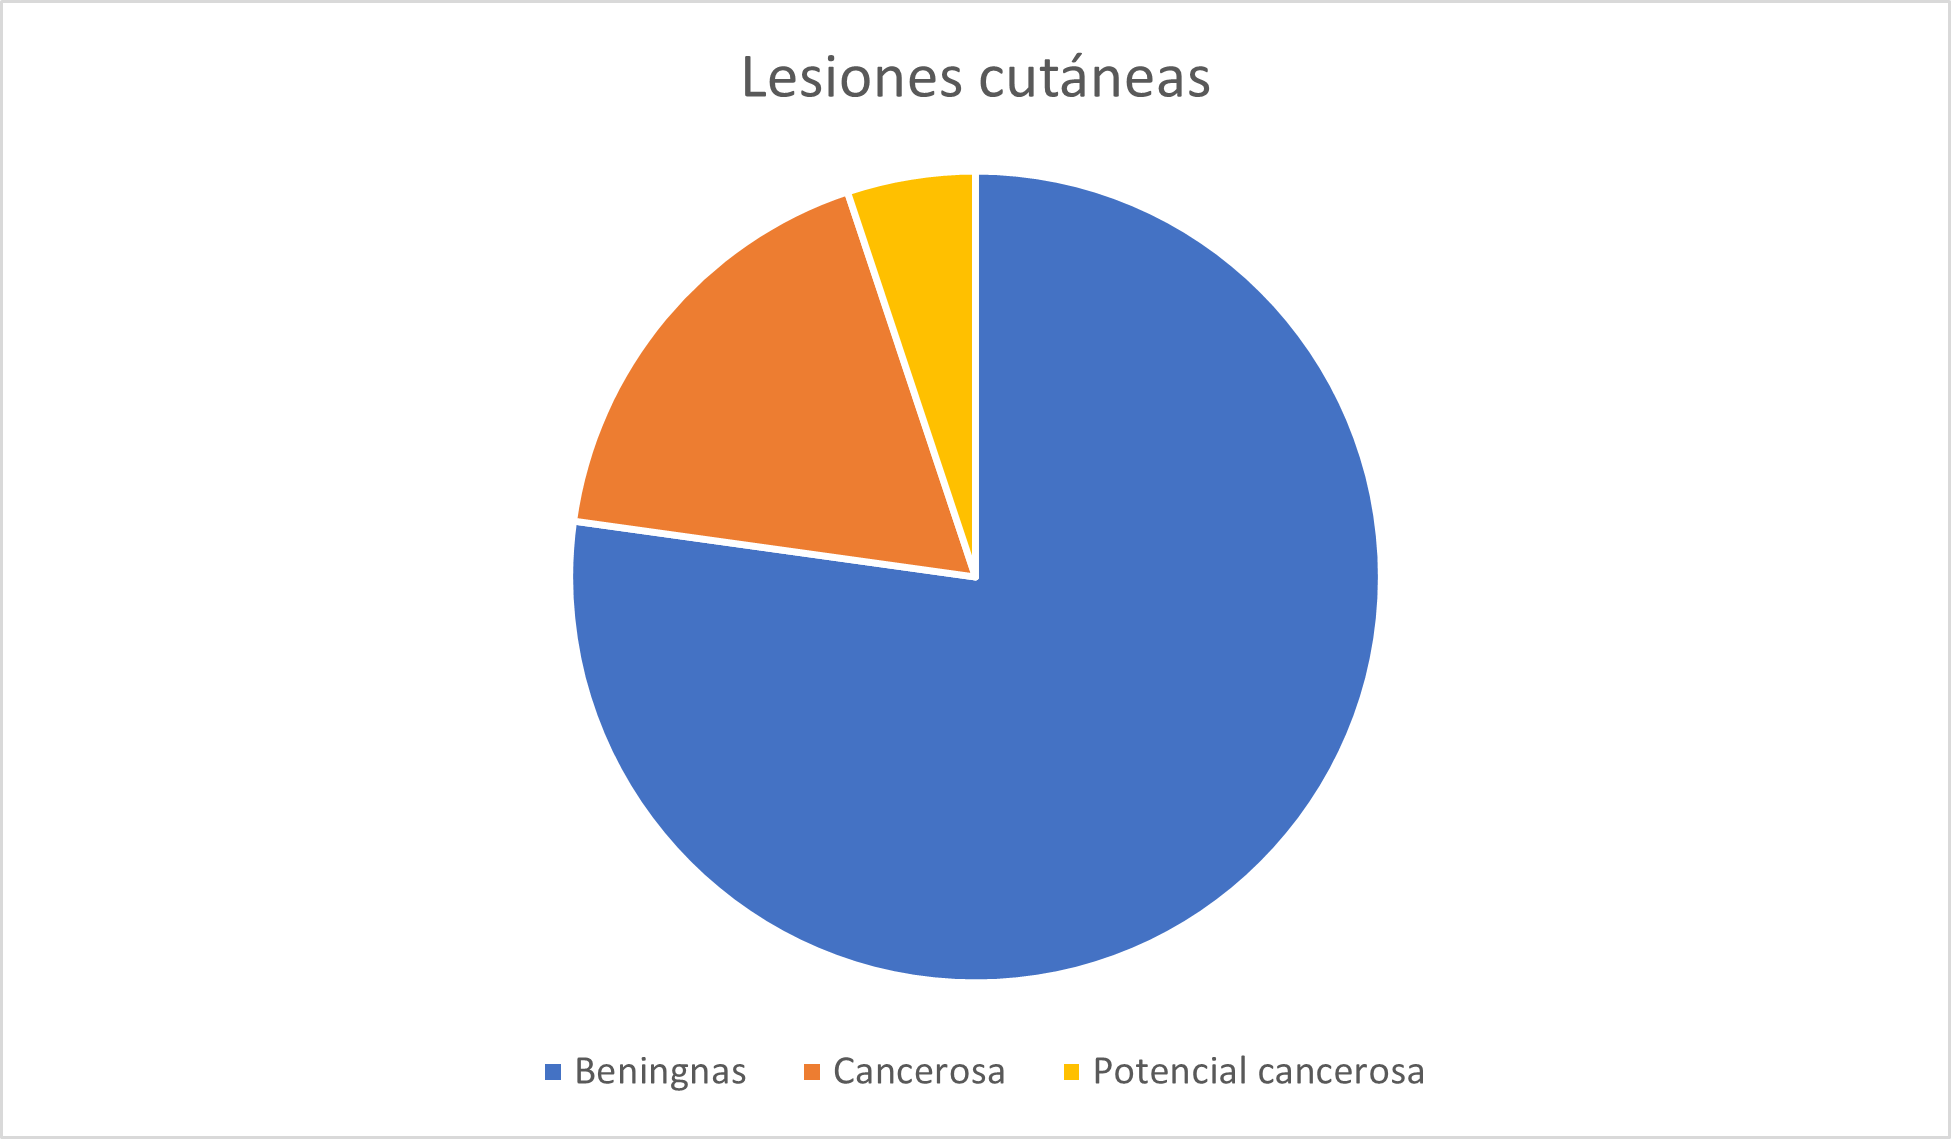
\includegraphics[scale = 0.65]{imagenes/datasetfinal.png}
	\caption{Distribución de clases}
\end{figure}

Se puede observar cómo la mayoría de imágenes disponibles engloban problemas de piel no cancerosos, mientras que el segundo tipo más común de lesión si es la cancerosa. Si atendemos a clasificar las subclases de cada tipo de patología, encontramos 52 posibles etiquetas.

%\section{Procesado de imágenes cutáneas}
%\subsection{Técnicas de reducción de ruido}
%\subsection{Normalización}
%\subsection{Extracción de características}


